\section{Count of persons data}
This section discusses the properties of the recorded datat as well as its suitability for context prediction.
\subsection{Properties of the data}
\label{sec:PassengerDensityData}

In order to model the passenger density an understanding of the available data is necessary. In this section the data, visible pattern and other features are discussed.

Figure~\ref{fig:rawData_week} illustrates exemplary the available values of a camera and week. The PdG service times are visible due to the low passenger density level between 01:00 and 05:00 on weekdays.

The figure details the passenger density data observed by one particular out of the 20 installed CCTV cameras (indexed with ID 700).
Due to the acquisition process in which denstiy information is extracted from circular snippets 
\marginpar{
\begin{figure}%[htbp]
  \begin{center}
  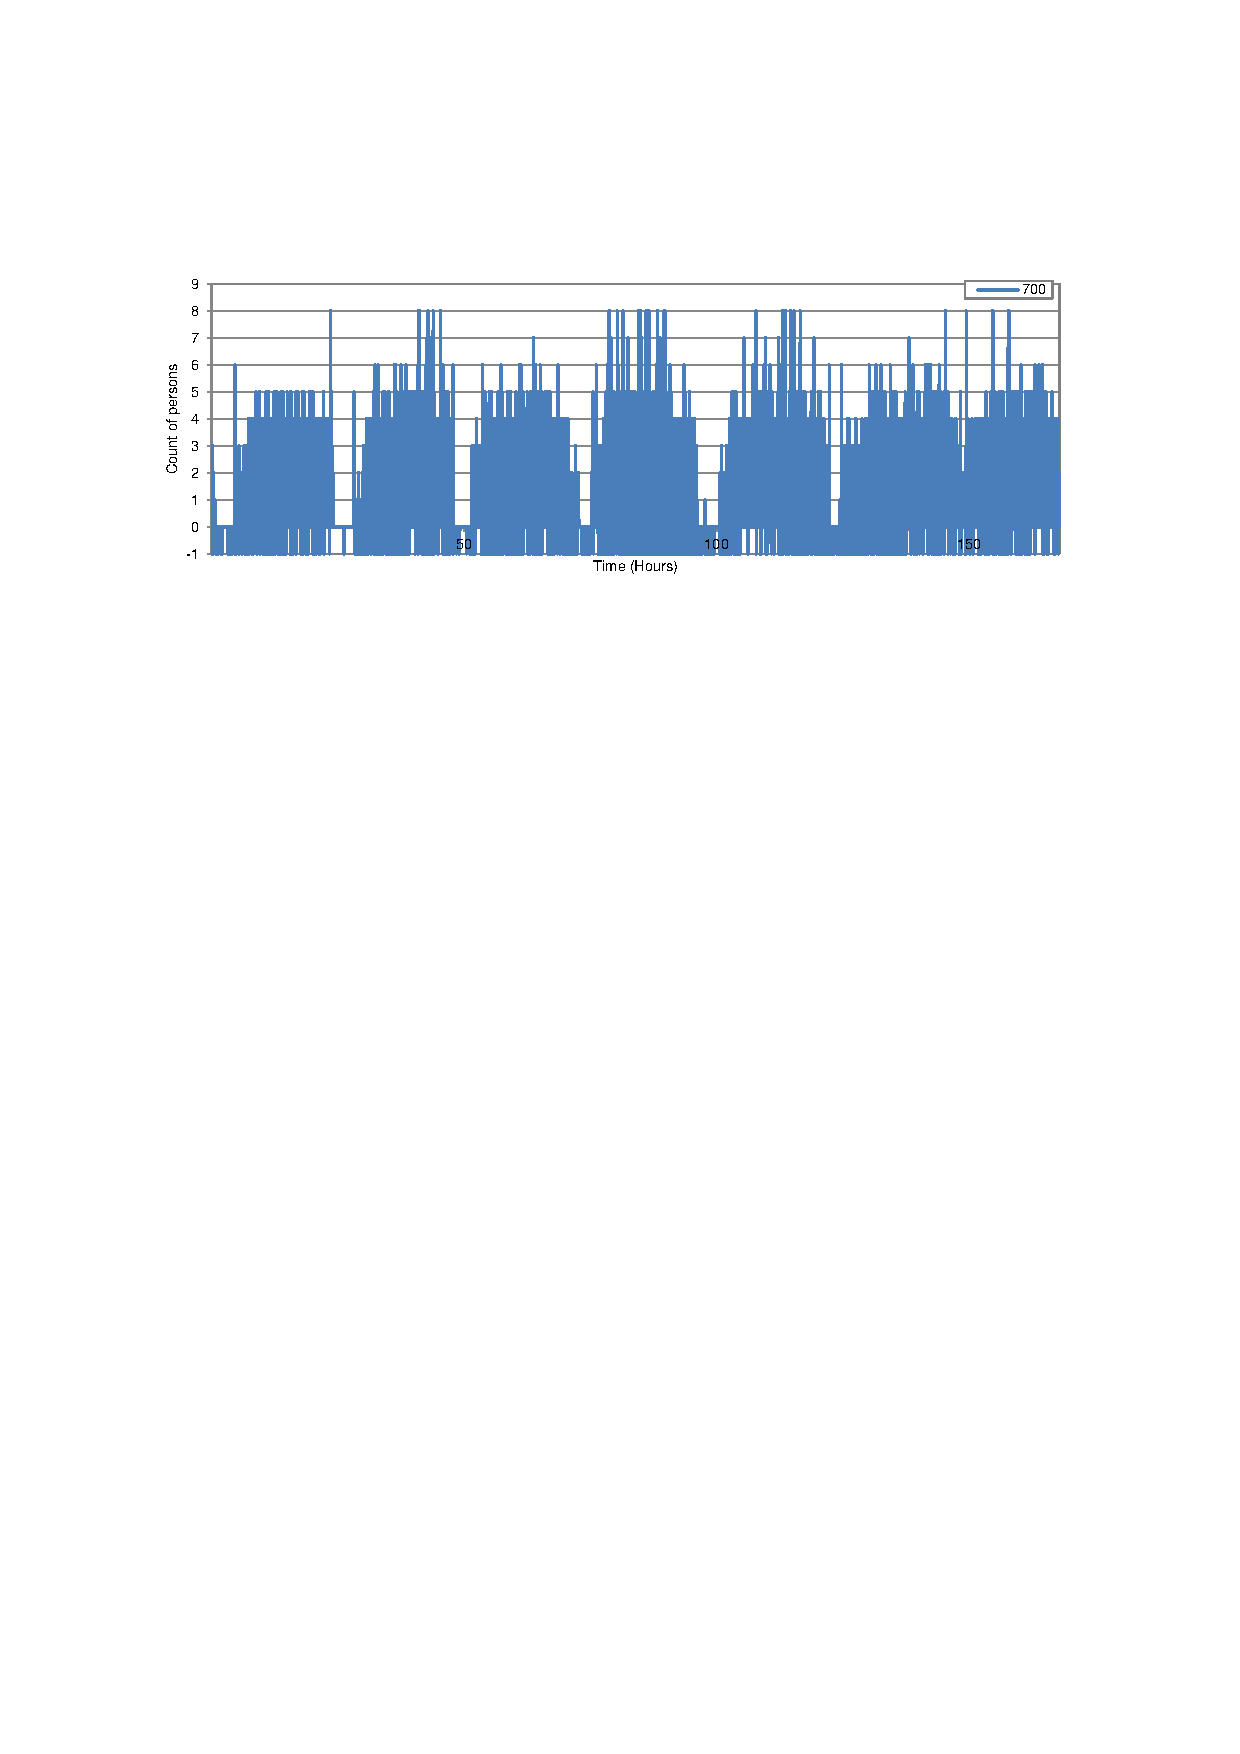
\includegraphics[height=\marginparwidth, angle=270]{Figures/rawData_week.pdf}
  \caption{Passenger density distribution of one camera during one week.}
  \label{fig:rawData_week}
  \end{center}
\end{figure}
}
of the various cameras (see description of the recording process above), for each camera one estimate on passenger density is computed every one minute, leading to a total of 1440 samples per camera and per day.
Again, due to the data processing operation, samples taken are not simultaneous for different cameras but taken sequentially so that pairwise samples are misaligned by at most 30 seconds.

\marginpar{
\begin{figure}
\begin{center}
 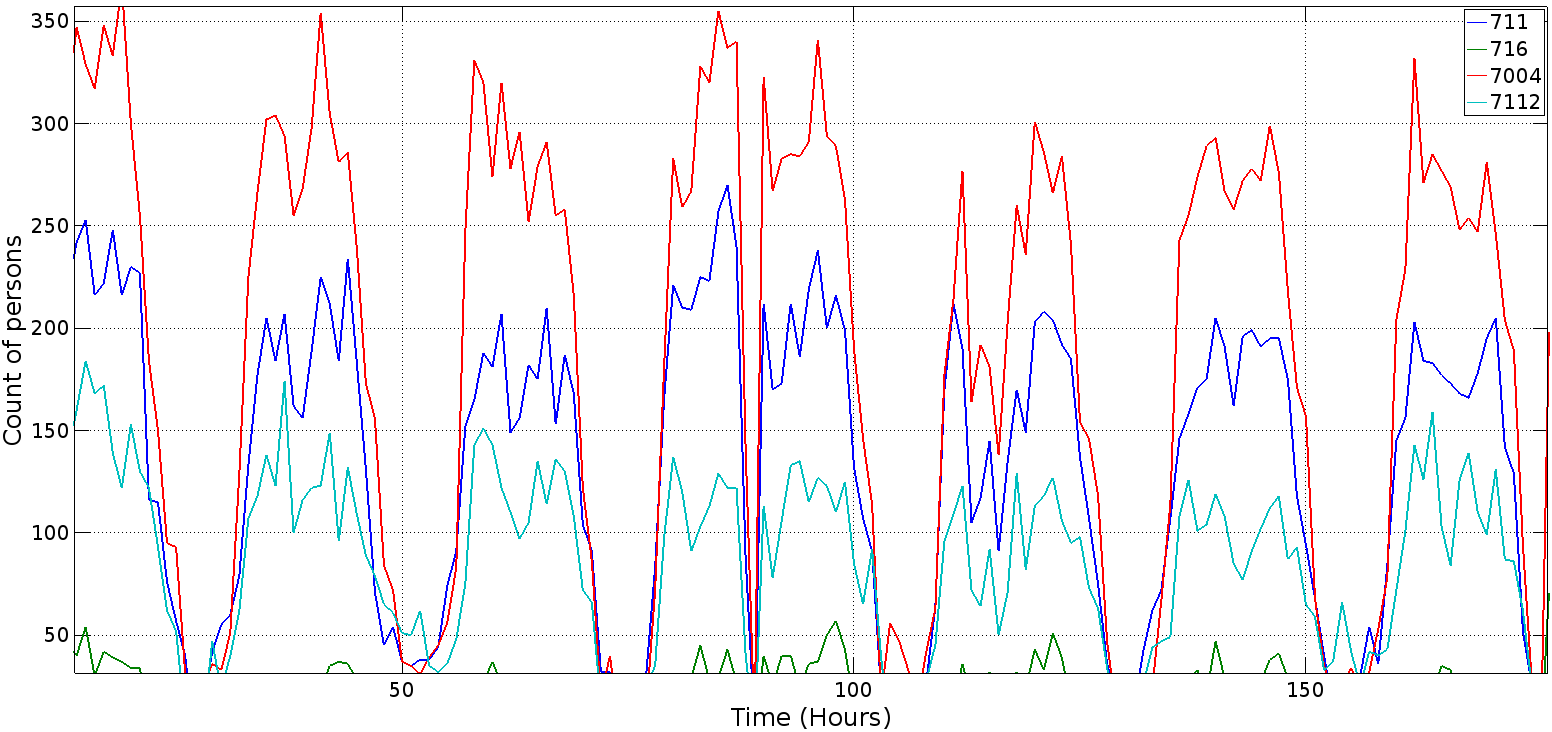
\includegraphics[height=\marginparwidth,angle=270]{Figures/Figure_PersonCount_Hours.png}
 \caption{todo}
  \label{figureHours}
  \end{center}
\end{figure}
}
\subsection{Prediction by Artificial Neural Fuzzy Inference System}

\begin{figure*}
\centering
     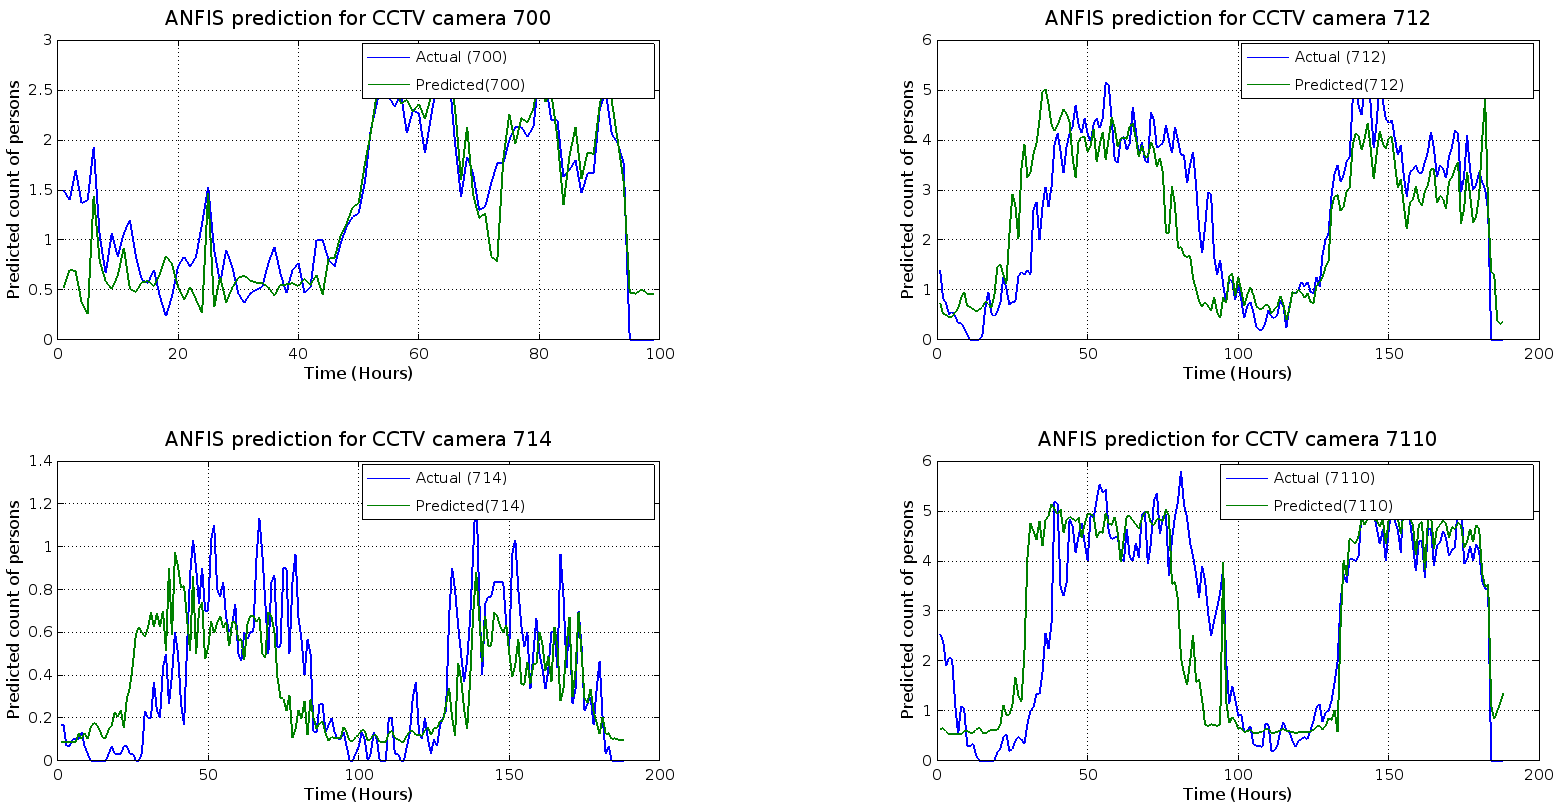
\includegraphics[width=\textwidth]{Figures/Figure_Prediction.png}
 \caption{todo}
\end{figure*}

\begin{figure*}
\centering
    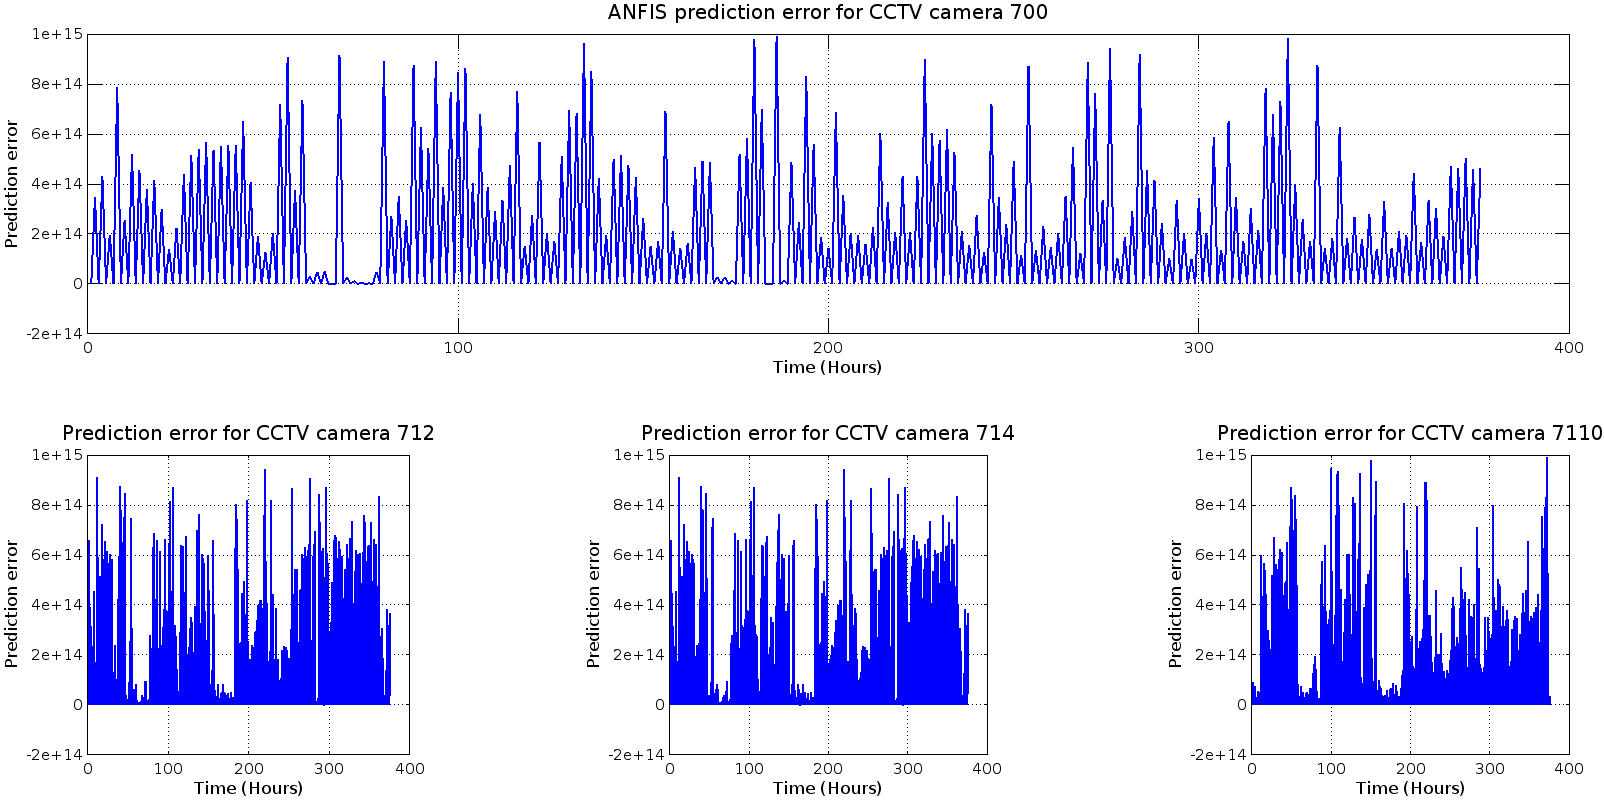
\includegraphics[width=\textwidth]{Figures/Figure_PredictionError.png}
 \caption{todo}
\end{figure*}

